\documentclass[conference]{IEEEtran}
\usepackage{amsmath,amssymb,graphicx,booktabs,url}
\usepackage[hidelinks]{hyperref}
\title{A Reproducible Simulation Benchmark of Reinforcement Learning and Classical Control for Electric Vehicle Battery Thermal Management}
\author{\IEEEauthorblockN{Rishuraj Singh, Nihaal Sansanwal, Harshit Singh Parmar, Chaitanya Sharma}
\IEEEauthorblockA{IILM University, Greater Noida, India}}
\begin{document}
\maketitle
\begin{abstract}Battery thermal management must balance temperature limits, spatial uniformity, auxiliary electricity, and a temperature-dependent aging proxy during driving and charging. We evaluate three continuous-action reinforcement learning controllers against tuned proportional-integral-derivative, bang-bang, null, and sampling model predictive control baselines in a four-node pack simulation. The electrical model is cross-checked against a published cell parameter set; thermal and cooling parameters remain assumptions. Five seeds per learning algorithm are trained for approximately 20,000 environment steps and evaluated on eight fixed episodes. The tuned proportional-integral-derivative controller obtains a mean shielded integrated cost of 1737.4, versus 1750.0, 1768.5, and 1841.6 for twin-delayed deep deterministic policy gradient, soft actor-critic, and proximal policy optimization. All supervised runs avoid the 15-45 $^{\circ}$C band violation, yet learned policies have mean episode intervention fractions of 19.6-22.7\%; without the supervisor their mean episode violation fractions are 41.2-42.3\%. One exported policy has 0.017 ms median laptop inference. At this training budget, learned controllers do not beat a fairly tuned simple baseline, and shielded reward alone conceals intrinsic safety weakness.\end{abstract}
\begin{IEEEkeywords}Battery thermal management, electric vehicles, reinforcement learning, safety supervision, comparative simulation.\end{IEEEkeywords}
\section{Introduction}
Temperature affects battery power, degradation, and cooling electricity. An electric-vehicle thermal controller must choose actions as battery current, ambient conditions, and charging change. Deep reinforcement learning offers a direct mapping from observations to continuous commands. A credible benefit claim, however, needs a tuned conventional baseline, fixed held-out scenarios, and explicit measurement of any supervisory override.

Prior work has applied reinforcement learning to combined battery and cabin cooling \cite{r1} and to joint fast charging and thermal control \cite{r2}. This work does not claim reinforcement learning itself is new to battery thermal management. Its narrower question is whether short-budget learned policies improve a shared objective against tuned proportional-integral-derivative (PID) control in an inspectable simulation, and how much of observed safety is supplied by an external override.

Soft actor-critic (SAC), twin-delayed deep deterministic policy gradient (TD3), and proximal policy optimization (PPO) were chosen because they directly handle the three continuous actuators and span stochastic off-policy, deterministic off-policy, and on-policy learning \cite{r3},\cite{r4},\cite{r5}. The contributions are a shared electrothermal plant and cost, separate raw and supervised evaluation, five training seeds per algorithm, and a policy-export runtime measurement. The central result is negative: at the recorded budget learned policies do not outperform tuned PID, and without the supervisor they violate the thermal band extensively.

Recent studies extend this context: Shin et al. investigate DDPG control of battery-subpack coolant flow and temperature against zone MPC \cite{r6}; Arjmandzadeh et al. study vehicle-level battery cooling during extreme fast charging with MPC and PID comparators \cite{r7}. Guo et al. examine hierarchical joint thermal-energy control under high ambient temperatures \cite{r8}, while Najmi et al. consider DRL with waste-heat recovery in cold hybrid fuel cell-battery powertrains \cite{r9}. These plants, operating regimes and objectives differ from ours; their reported benefits are not evidence of a benefit in this benchmark. The present contribution remains a limited-budget, auditable comparison with explicit raw-policy and supervisor-dependent outcomes. This targeted literature update was checked on 27 October 2026 and is not an exhaustive systematic review.

\section{Plant And Control Problem}
\subsection{Drive load and electrical dynamics}
Official one-hertz speed schedules are transformed into traction demand using vehicle mass 1800 kg, drag coefficient 0.28, frontal area 2.3 m2, rolling coefficient 0.01, 90\% drivetrain efficiency, bounded regenerative braking, and a 700 W accessory load. These describe an assumed vehicle, not an identified production car. With acceleration a and road-grade fraction g\_r, define theta=arctan(g\_r). The exact implemented road-load force is

\begin{equation}
\begin{gathered}F_t=m\dot v+mgC_r\cos\theta+mg\sin\theta\\\quad+\frac{1}{2}\rho C_d A v^2,\qquad\theta=\arctan g_r\end{gathered}
\label{eq:1}
\end{equation}
The source speed schedules are urban UDDS, highway HWFET, aggressive US06, and NEDC assembled from four ECE segments and one EUDC segment \cite{r10}. They provide speed versus time; grade, ambient temperature, pack parameters, and charging are separate simulation inputs.

The 96-series/34-parallel pack has nominal capacity 170 Ah and a first-order Thevenin electrical model. Open-circuit voltage V\_oc depends on state of charge z; ohmic resistance R\_0 depends on z and temperature T. One polarization branch has resistance R\_1 and time constant tau. Positive current denotes discharge:

\begin{equation}
\begin{gathered}V_t=V_{\mathrm{oc}}(z)-IR_0(z,T)-v_{\mathrm{RC}}\\\dot z=-I/(3600Q_{\mathrm{Ah}})\end{gathered}
\label{eq:2}
\end{equation}
The polarization state follows dv\_RC/dt=(I R\_1-v\_RC)/tau. Resistive heat is I\textasciicircum{}2 R\_0 plus v\_RC\textasciicircum{}2/R\_1; the latter is integrated through each constant-current substep, so temporary capacitor storage is not treated as immediate heat. Open-circuit voltage and pulse resistance were cross-checked at four states of charge against Chen et al.'s cell parameter set \cite{r11} in a single-particle model with electrolyte (SPMe) \cite{r12} implemented with PyBaMM \cite{r13}. The 30 s time constant, temperature coefficient, and pack-scale extrapolation remain assumptions. This cross-check is not physical pack validation.

\subsection{Four-node thermal and finite-coolant model}
Four equal thermal nodes, each 60 kJ/K, exchange heat with neighbors, ambient air, and coolant that warms serially as it passes the nodes. Each node receives one quarter of electrical heat generation. A 20 kJ/K finite coolant inventory receives node and pump heat; radiator rejection and a powered chiller remove heat. This avoids an implicit unlimited fixed-temperature cooling source and permits an energy-accounting check.

The control vector a=(pump, fan, chiller) lies in [0,1]\textasciicircum{}3. Assumed maxima are 0.5 kg/s coolant flow and 12 kW chiller removal at coefficient of performance 2.5. Pump and fan electricity are 150 pump\textasciicircum{}3 and 300 fan\textasciicircum{}3 W, respectively. Active cooling requires circulation. The four-node structure resolves spatial spread but not cell-scale gradients, detailed pack geometry, or thermal runaway.

\subsection{Observation, objective, and supervisor}
The controller acts every 5 s and the plant integrates at 1 s. Its 12-element observation contains four node temperatures, state of charge, C-rate, ambient temperature, driving or charging mode, coolant temperature, current demand, 30 s mean demand, and 60 s maximum demand. Episodes stop at their set duration or if state of charge leaves (0.05,0.95).

Every controller minimizes the same time-integrated cost. At each second, d is exceedance above 45 $^{\circ}$C plus exceedance below 15 $^{\circ}$C, Delta T is node maximum minus minimum, E\_aux is auxiliary joules, and A is a relative aging-severity increment. The implemented one-second cost is

\begin{equation}
c_t=20(d_t/5)^2+\Delta T_t/5+E_{\mathrm{aux},t}/3000+A_t/5
\label{eq:3}
\end{equation}
Episode cost J is the sum of c. The aging quantity is a model-derived exposure proxy, not measured capacity fade or remaining life. The normalized cost is not watt-hours or degradation percent. Auxiliary watt-hours and violation seconds are therefore also reported.

An optional heuristic supervisor overwrites all three actions with full cooling when maximum node temperature reaches 42 $^{\circ}$C, checking each one-second plant substep. The evaluation band is 15-45 $^{\circ}$C. It has no formal safety guarantee. We report how often it fires and test raw controllers separately with it disabled.

\begin{table}[t]
\caption{Selected assumed plant and control parameters.}
\label{tab:I}
\centering\footnotesize
\begin{tabular}{lr}
\toprule
Parameter & Value\\
\midrule
Pack & 96s34p, 170 Ah\\
Thermal nodes & 4 $\times$ 60 kJ/K\\
Coolant capacity & 20 kJ/K\\
Maximum flow & 0.5 kg/s\\
Chiller / COP & 12 kW / 2.5\\
Physics / control & 1 s / 5 s\\
Band / trigger & 15-45 $^{\circ}$C / 42 $^{\circ}$C\\
\bottomrule
\end{tabular}
\end{table}
\section{Experiment Design}
\subsection{Fixed scenarios and validation gates}
The eight held-out episodes comprise two mild UDDS cases at 25 $^{\circ}$C ambient, two repeated-US06 hot cases at 43 $^{\circ}$C and 6\% grade, two specified 2C fast-charge cases at 38 $^{\circ}$C, one NEDC case at 45 $^{\circ}$C, and one HWFET case at 30 $^{\circ}$C. Principal-scenario seeds perturb initial state of charge and temperature; they are not independent physical packs. Charging tapers above 80\% state of charge and is limited to a modeled 4.2 V per series cell.

\begin{table}[t]
\caption{Fixed held-out evaluation manifest.}
\label{tab:II}
\centering\footnotesize
\begin{tabular}{lrr}
\toprule
Input & Cases & Duration\\
\midrule
UDDS mild & 2 & 1365 s\\
US06 hot & 2 & 1800 s\\
2C charge & 2 & 1350 s\\
NEDC hot & 1 & 1180 s\\
HWFET mild & 1 & 765 s\\
\bottomrule
\end{tabular}
\end{table}
A pretraining hardness gate verifies that cooling matters. With cooling disabled, the mild case has no thermal-band violation; hot driving exceeds the band for 1472/1800 s and fast charging for 1181/1350 s. Full cooling avoids violation in the hot and charging gates. Uncontrolled maxima of 53.0 and 81.0 $^{\circ}$C are simulated outputs, not real-pack predictions. Ten recorded plant and environment checks passed. Modeled driving-demand values, including drivetrain/regen efficiency and accessories but excluding pack-internal losses and BTMS power, are 13.26, 13.30, 18.74, and 13.99 kWh/100 km for UDDS, HWFET, US06, and NEDC.

\subsection{Learning and baseline configuration}
Each SAC, TD3, and PPO policy uses a two-layer 64-by-64 multilayer perceptron, learning rate 3e-4, eight CPU environments, five random seeds, and a nominal 20,000-step budget. SAC and TD3 use a 200,000-transition replay buffer, batch size 256, and 2000 warm-up steps. PPO uses 256 rollout steps per environment and ten update epochs, reaching the next rollout boundary at 20,480 steps. Observation normalization is calibrated away from the held-out set and frozen for deterministic final inference. Training-time evaluations use a tuning split.

PID is tuned on the same cost with the supervisor enabled, across 18 combinations of setpoint 30/35/39 $^{\circ}$C, proportional gain 0.1/0.3/0.6, integral gain 0/0.002, and zero derivative gain. The selected configuration is 39 $^{\circ}$C, Kp=0.6, Ki=Kd=0. Null and bang-bang controllers are additional baselines. Sampling model predictive control (MPC) chooses among ten candidate actions over a 12-step, 60 s horizon using the nominal plant; it is not an exact optimum.

All controllers replay the same eight test episodes. Each nonlearning baseline has one eight-episode result; each learned seed replays all eight. The episodes were constructed rather than sampled from a vehicle population. In the saved comparison plot, baseline error bars reflect episode variation, while learned-policy error bars reflect variation among five seed-level episode means; they are not comparable confidence intervals.

Percentages are first calculated per episode, then averaged with equal episode weights; learned-policy summaries additionally average the five seed-level episode means. Different episode durations therefore do not give longer episodes larger weights. A reported mean percentage is not the pooled fraction of all simulated seconds.

\begin{figure}[t]
\centering
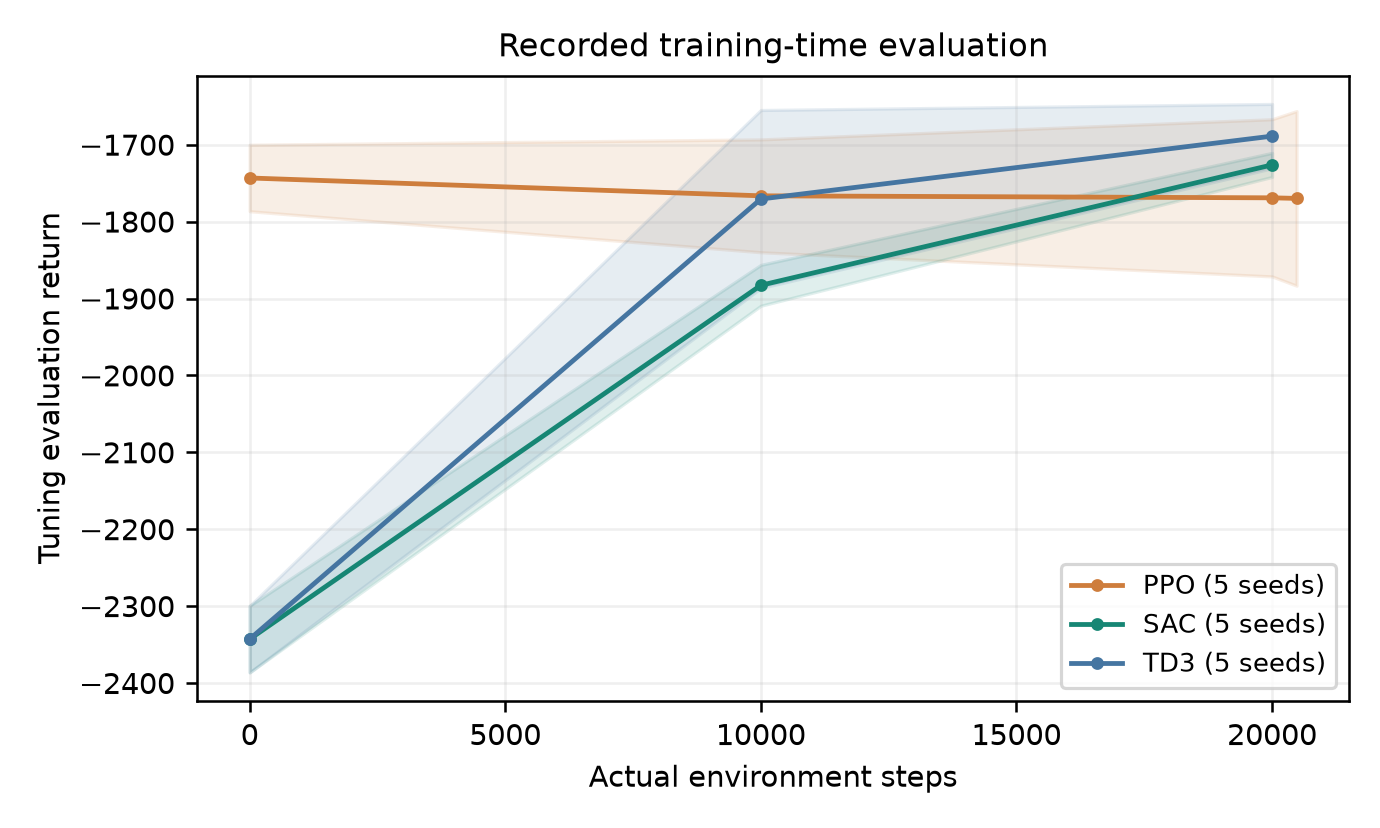
\includegraphics[width=\columnwidth]{../report/paper_revision/figures/figure_1.png}
\caption{Tuning-split evaluation return during training (higher is better). Lines are five-seed means, with between-seed spread. This is not the final held-out test.}
\label{fig:1}
\end{figure}
The training trace shows SAC and TD3 improving on the tuning split between initialization and 20,000 steps, while PPO changes less. Progress on the tuning split does not imply improvement over PID on held-out episodes.

\section{Held-Out Results}
\subsection{Supervised controller comparison}
Sampling MPC has the lowest mean supervised cost, 1618.4. Tuned PID reaches 1737.4, outperforming TD3 by 12.7 cost units (0.7\% of PID cost), SAC by 31.1 (1.8\%), and PPO by 104.2 (6.0\%). These are descriptive differences across five trained seeds and eight fixed simulated episodes; they are not population-level significance claims. Null control with the same supervisor scores 1776.1, close to SAC, emphasizing the override's contribution.

\begin{table}[t]
\caption{Held-out shielded means; percentages average episodes equally.}
\label{tab:shielded}
\centering\footnotesize
\begin{tabular}{lrrr}
\toprule
Controller & Cost & Aux. Wh & Fire \%\\
\midrule
Sampling MPC & 1618.4 & 445.3 & 14.31\\
Tuned PID & 1737.4 & 482.3 & 1.23\\
TD3 & 1750.0 & 484.0 & 21.85\\
SAC & 1768.5 & 490.4 & 19.63\\
PPO & 1841.6 & 474.8 & 22.70\\
Null with shield & 1776.1 & 473.8 & 22.68\\
Bang-bang & 1983.1 & 626.8 & 1.23\\
\bottomrule
\end{tabular}
\end{table}
\begin{figure}[t]
\centering
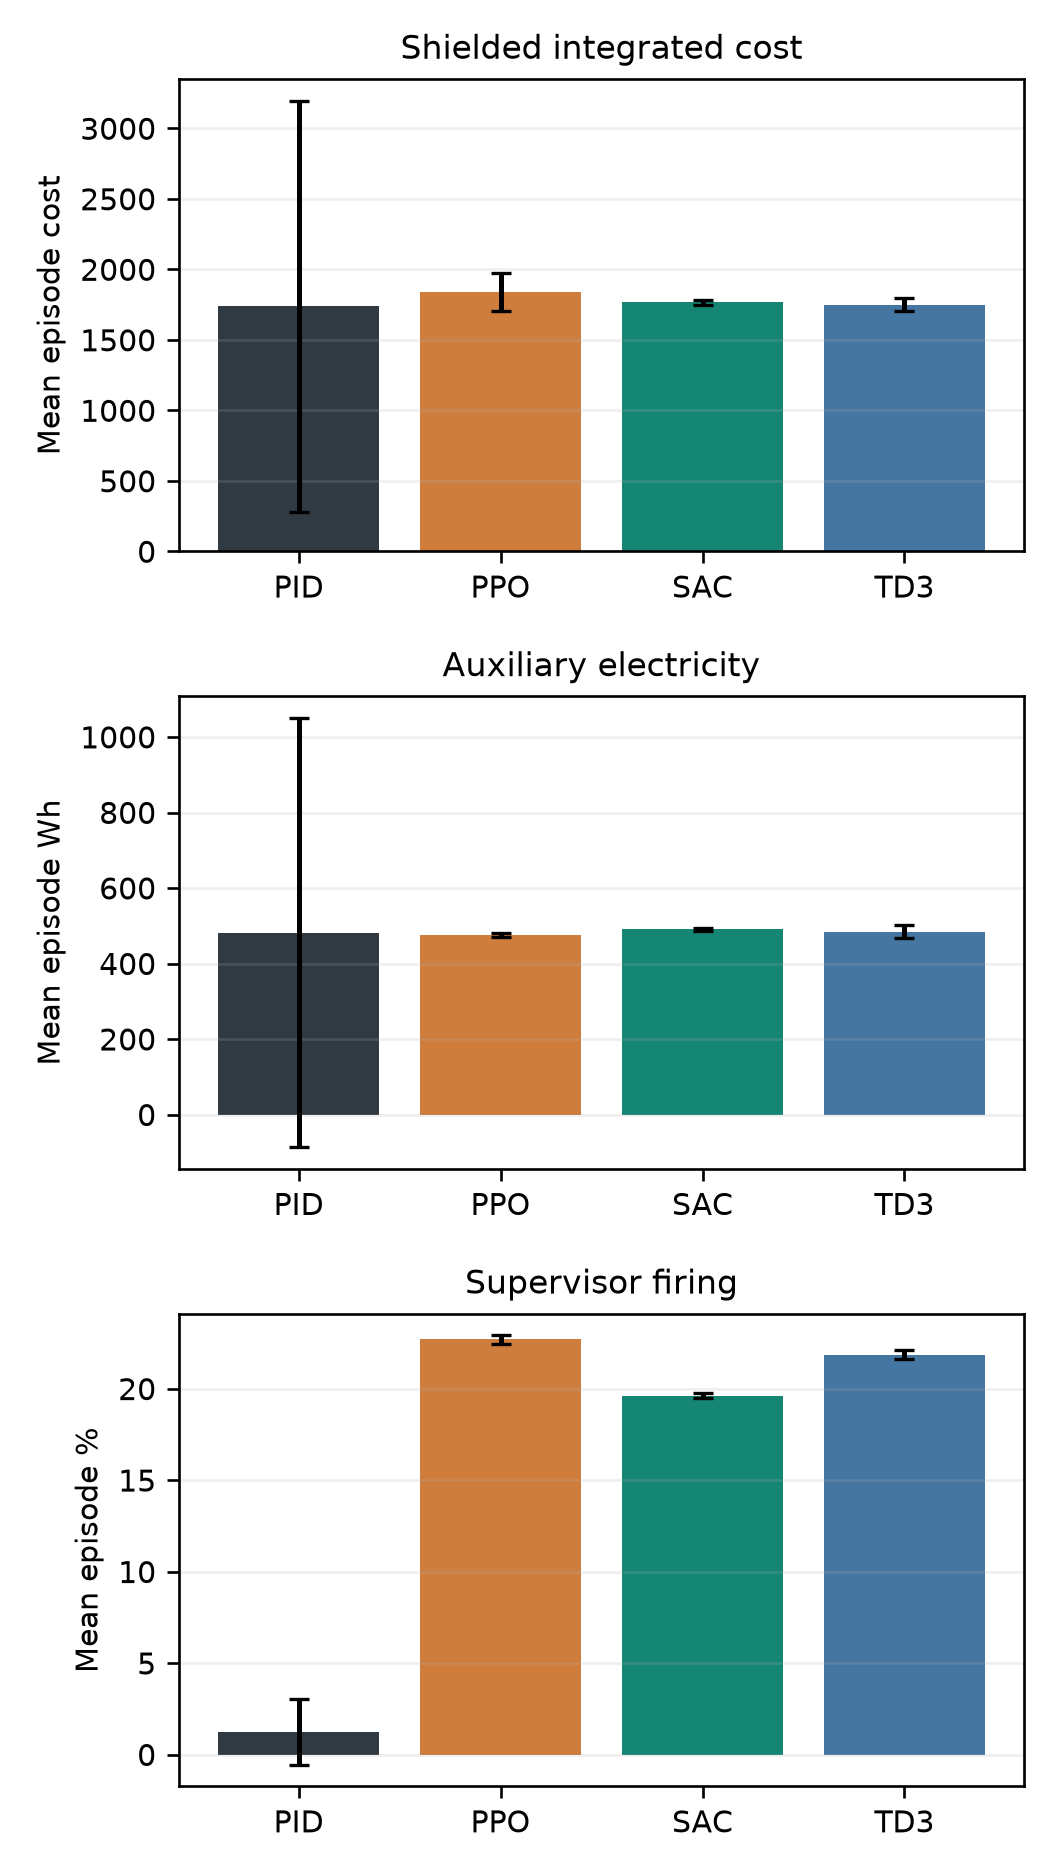
\includegraphics[width=\columnwidth]{../report/paper_revision/figures/figure_2.png}
\caption{Saved three-panel comparison of supervised cost, auxiliary energy, and shield firing. Baseline and learned-policy error bars have different definitions, so the figure is descriptive rather than an equal-meaning uncertainty comparison.}
\label{fig:2}
\end{figure}
\begin{figure}[t]
\centering
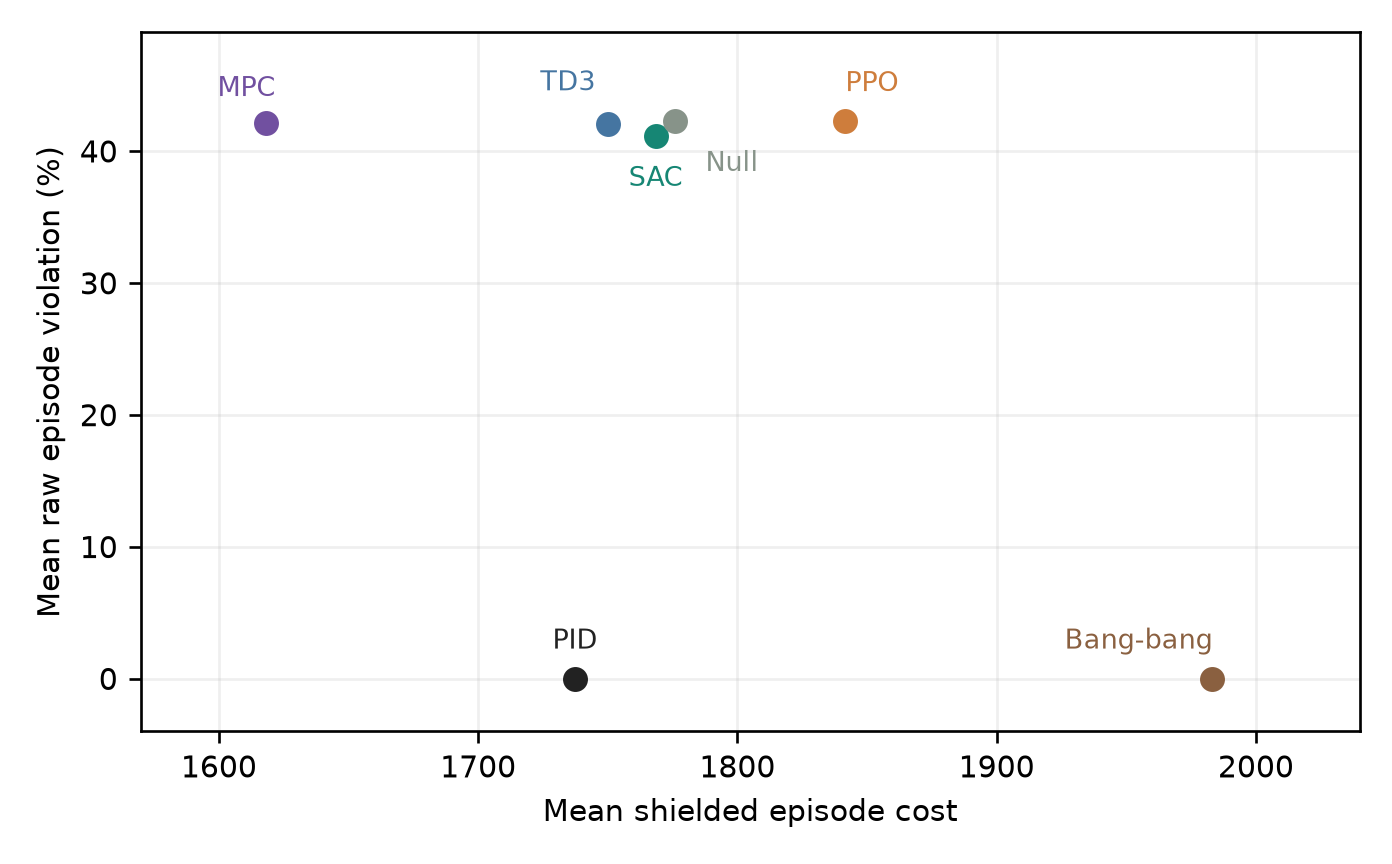
\includegraphics[width=\columnwidth]{../report/paper_revision/figures/figure_3.png}
\caption{Mean shielded cost versus mean episode raw band-violation percentage for all seven controllers, using separate rollouts. PID and bang-bang both record zero raw violation; these are outcomes on the fixed manifest, not safety certificates.}
\label{fig:3}
\end{figure}
All supervised controllers avoid band violations on the fixed manifest. This does not make their proposed actions independently safe. The supervisor fires with mean episode firing fractions of 1.23\% for PID and 19.63-22.70\% for the learned policies. PPO uses slightly less auxiliary electricity than PID yet has higher total cost and much more intervention, illustrating why energy alone cannot determine controller ranking.

\subsection{Raw-policy safety}
\begin{table}[t]
\caption{Raw held-out control; violation percentages average episodes equally.}
\label{tab:raw}
\centering\footnotesize
\begin{tabular}{lrr}
\toprule
Controller & Cost & Viol. \%\\
\midrule
Tuned PID & 1735.4 & 0.00\\
Bang-bang & 1983.1 & 0.00\\
Sampling MPC & 2897.6 & 42.15\\
SAC & 54951.4 & 41.15\\
TD3 & 105270.1 & 42.08\\
PPO & 140570.3 & 42.28\\
Null & 144062.8 & 42.28\\
\bottomrule
\end{tabular}
\end{table}
Without the override, the learned controllers have mean episode band-violation fractions of 41.15-42.28\%. Their costs rise sharply because the band penalty is quadratic. PID and bang-bang show zero raw violation on this manifest; PID cost changes only from 1735.4 raw to 1737.4 supervised. Raw sampled MPC has a mean episode violation fraction of 42.15\%, so its favorable supervised cost does not establish independent safety.

\begin{figure}[t]
\centering
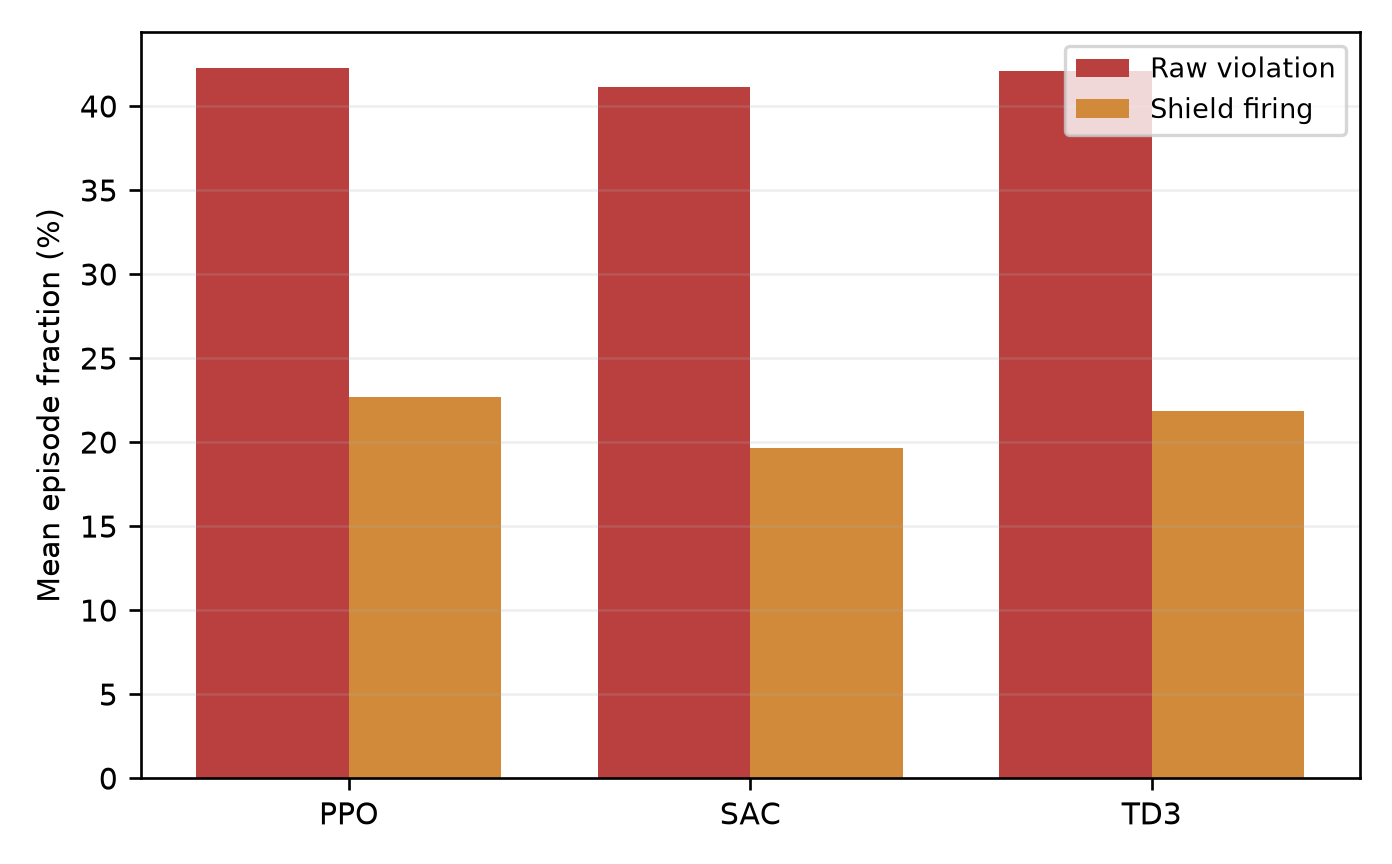
\includegraphics[width=\columnwidth]{../report/paper_revision/figures/figure_4.png}
\caption{Mean episode raw band-violation percentage (red) and mean episode supervisor firing percentage in separate shielded rollouts (orange). Episodes are equally weighted; these bars neither pool all seconds nor partition one rollout.}
\label{fig:4}
\end{figure}
\begin{figure}[t]
\centering
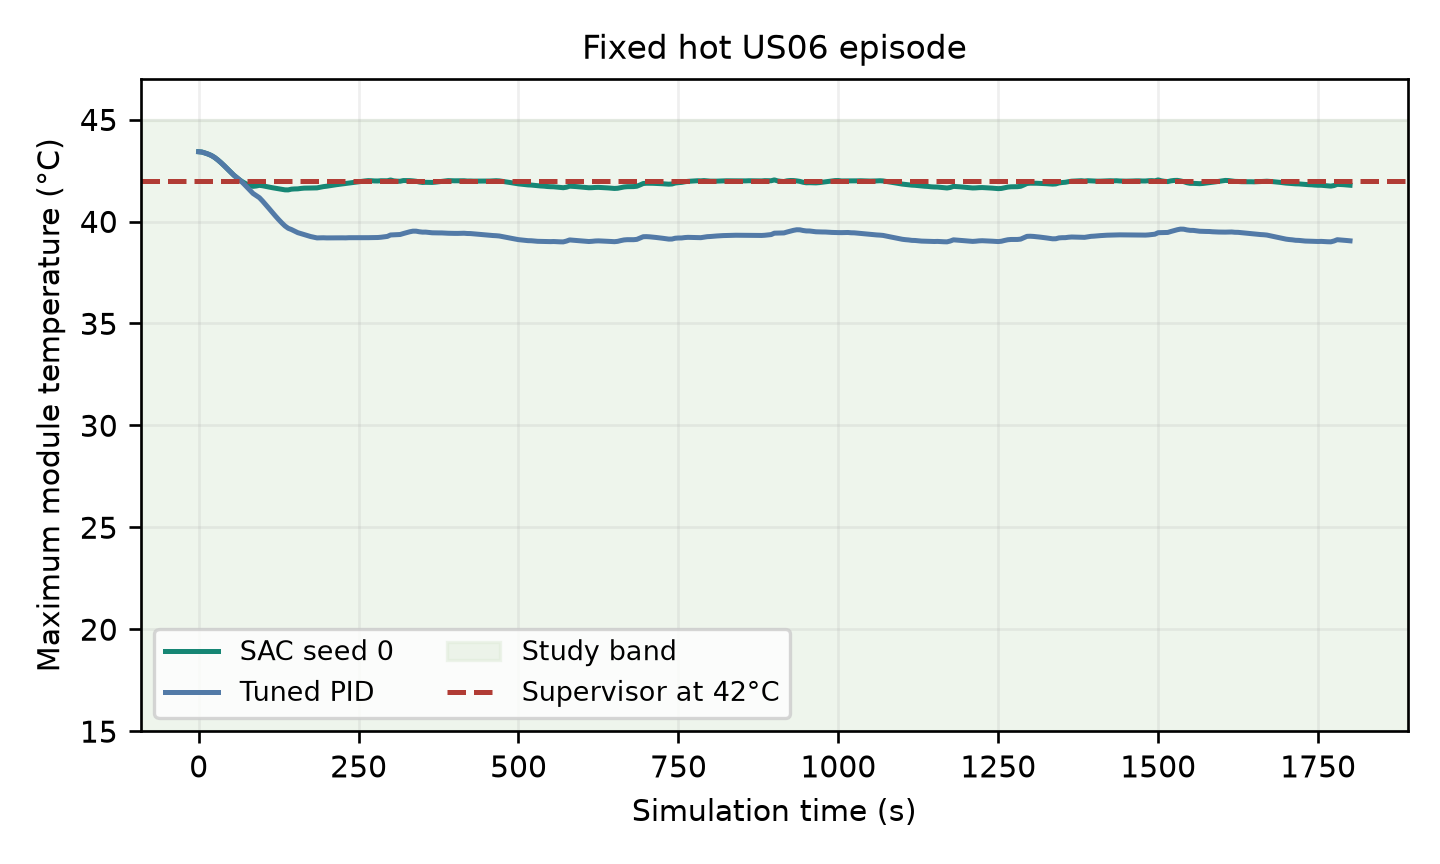
\includegraphics[width=\columnwidth]{../report/paper_revision/figures/figure_5.png}
\caption{Representative hot US06 episode with supervisor enabled. The saved SAC seed-zero and tuned-PID maximum-node temperatures remain within the shaded 15-45 $^{\circ}$C band; the dashed line is the 42 $^{\circ}$C shield trigger.}
\label{fig:5}
\end{figure}
For SAC seed zero, intervention is roughly 12-13\% of hot US06 seconds and 63-65\% of fast-charge seconds, but zero in the two mild UDDS and HWFET cases. Dependence on the supervisor is concentrated in demanding conditions. Zero observed violations under this plant and manifest are not proof that the 42 $^{\circ}$C trigger always provides sufficient margin.

\section{Runtime And Deployment Boundary}
One SAC seed-zero actor was exported to ONNX and dynamically quantized to INT8. On a 13th-generation Intel Core i5-13420H laptop CPU, 500 warmed inference calls on the same fixed observation yield median/99th-percentile times of 0.017/0.0256 ms for ONNX, 0.0217/0.0328 ms for INT8, and 0.092/0.190 ms for PyTorch. ONNX and INT8 files occupy 24.94 and 16.04 KiB; maximum absolute action differences over three components at that one observation are 2.98e-8 and 0.00142. Sampling MPC takes 228.95/288.85 ms over 50 solves on the same laptop.

The benchmark warms each inference function before its timed fixed-observation calls. Its maximum action-error statistic covers three actuator components at that one initial hot-state observation, not a trajectory-wide or worst-case error bound. The deployment artifact also retains separate eight-episode shielded evaluations of ONNX and INT8 policies. One KiB denotes 1024 bytes.

\begin{table}[t]
\caption{Recorded warmed fixed-observation laptop timing.}
\label{tab:V}
\centering\footnotesize
\begin{tabular}{lrrr}
\toprule
Runtime & Median ms & P99 ms & Calls\\
\midrule
PyTorch & 0.0920 & 0.1899 & 500\\
ONNX & 0.0170 & 0.0256 & 500\\
INT8 & 0.0217 & 0.0328 & 500\\
MPC & 228.95 & 288.85 & 50\\
\bottomrule
\end{tabular}
\end{table}
\begin{figure}[t]
\centering
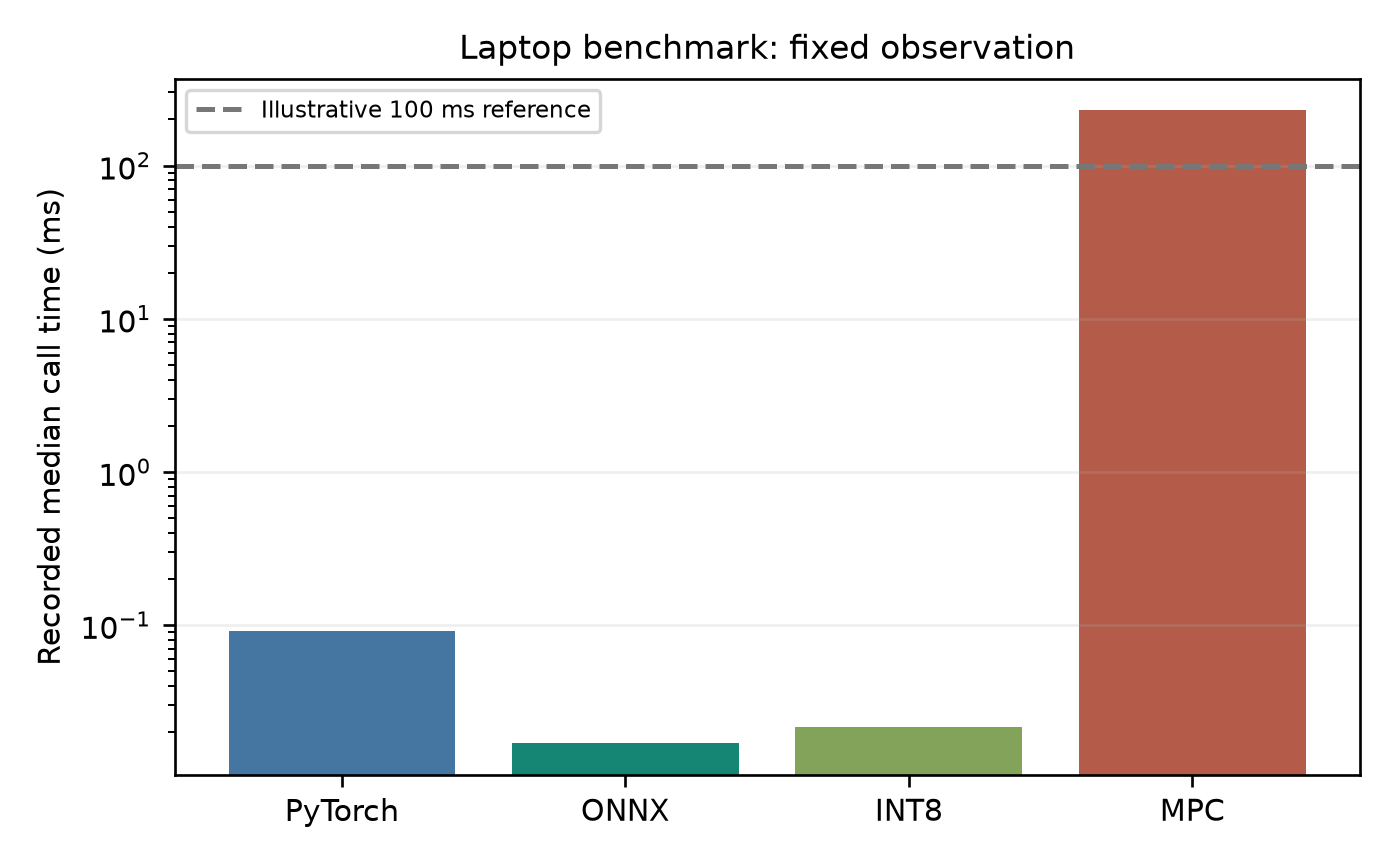
\includegraphics[width=\columnwidth]{../report/paper_revision/figures/figure_6.png}
\caption{Laptop median inference or solve time on a logarithmic scale. The 100 ms line is an illustrative 10 Hz budget; simulated control updates every 5 s.}
\label{fig:6}
\end{figure}
The measurements establish computational headroom on this laptop only. They are not automotive electronic-control-unit measurements, a worst-case execution-time certificate, or roadworthiness evidence. Policy inference and MPC solve calls are different tasks; timing does not equal control quality.

\section{Interpretation And Limitations}
Three propositions remain distinct: a neural actor can execute quickly on this laptop; a common supervisor keeps these particular simulated trajectories inside the chosen band; and a controller may or may not improve the integrated objective. The first two do not imply the third, nor intrinsic policy safety. Here raw learned control fails the safety test and supervised learned cost does not beat tuned PID.

The null-with-supervisor cost, 1776.1, is only 38.7 above PID and 7.6 above SAC. This does not prove the learned policy has no useful effect in every episode; it demonstrates that aggregate supervised cost alone is a weak measure of what the policy learned. Full-cooling overrides can dominate hot states. Future work should report paired per-scenario costs, command distributions, intervention-conditioned outcomes, preview ablations, longer and compute-matched training, and robustness to uncertain ambient and pack parameters.

The plant is reduced order and largely assumption driven. The published-cell comparison covers selected electrical points, not a measured pack or thermal circuit. Four equal thermal capacities, conductances, chiller and pump curves, grade, simplified 2C charging, and the aging proxy can change controller rankings. The eight designed episodes are not a representative fleet. The same nominal plant supports control and evaluation, so model mismatch is untested. No hardware-in-the-loop, pack experiment, fault injection, sensor-delay study, or thermal-runaway assessment was performed. Five seeds do not justify broad statistical claims.

\section{Detailed Model Specification}
\subsection{Source cycles, traction demand, and charging}
The cycle loader retains provenance metadata and hashes for the downloaded speed traces. UDDS is the urban dynamometer driving schedule; HWFET is the highway fuel economy test; US06 emphasizes aggressive acceleration. ECE is the urban European segment and EUDC its extra-urban companion; the assembled NEDC comprises four ECE segments and one EUDC with duplicate shared endpoints removed. The imported files are one-hertz speed schedules, not records of battery current, temperature, or cooling electricity. All such battery variables come from the simulated vehicle and pack. The source-cycle duration may differ slightly from an episode, because the episode specifies its own horizon and can repeat the speed trace.

\begin{table}[t]
\caption{Source speed data and modeled demand, including drivetrain assumptions.}
\label{tab:VI}
\centering\footnotesize
\begin{tabular}{lrrr}
\toprule
Cycle & s & km & kWh/100 km\\
\midrule
UDDS & 1369 & 11.99 & 13.26\\
HWFET & 765 & 16.51 & 13.30\\
US06 & 600 & 12.89 & 18.74\\
NEDC & 1180 & 10.93 & 13.99\\
\bottomrule
\end{tabular}
\end{table}
At each second, finite differences of speed provide acceleration. In addition to the traction terms in (1), drivetrain efficiency modifies positive road-load power; regenerative power is bounded and scaled by the assumed recovery efficiency. The 700 W accessory load and thermal-system electrical draw then enter pack power demand. The electrical model solves current from terminal power through the Thevenin relationship. This creates an important coupling: more cooling consumes energy, which changes battery current and therefore heat generation. During charging, the current request is initially -2 times nominal ampere-hour capacity in amperes. The request tapers linearly from 80\% to 90\% state of charge and obeys the 4.2 V-per-series-cell terminal-voltage limit. No electrochemical plating constraint is modeled.

\subsection{Electrical heat and state accounting}
For the polarization branch, the exact constant-current update is v\_RC(t+dt)=I R\_1+[v\_RC(t)-I R\_1] exp(-dt/tau). The heat sent into the thermal nodes is the ohmic integral plus the resistor's v\_RC squared over R\_1 integral. This is distinct from treating I squared R\_1 as heat throughout a current transient: some branch input first becomes capacitor energy. The nominal reference values include R\_1 about 0.0434 ohm and an assumed 30 s time constant; R\_0 varies with state of charge and temperature. The charge sign convention and state-of-charge update use the same 170 Ah pack capacity throughout.

\begin{equation}
v_{\mathrm{RC}}(t+\Delta t)=IR_1+[v_{\mathrm{RC}}(t)-IR_1]e^{-\Delta t/\tau}
\label{eq:4}
\end{equation}
The source parameter comparison uses the published Chen et al. cell parameterization at four selected states of charge, with pack scaling for 96 series and 34 parallel cells. It checks open-circuit voltage and equivalent pulse resistance at those points. It cannot validate the four-node thermal capacities, coolant path, pack contact resistances, or behavior outside the sampled state-of-charge and temperature region. The recorded cell-only thermal mass is approximately 139.6 kJ/K, while this study's four-node pack has 240 kJ/K; the additional hardware mass is an explicit assumption, not a derived cell measurement.

\subsection{Thermal flow and actuator laws}
Neighbor conduction uses 12 W/K between adjacent nodes, ambient exchange 4 W/K per node, and a nominal 250 W/K coolant exchange coefficient per node. The coolant enters node 1, warms after each node's heat transfer, and reaches downstream nodes at a different temperature. For flow m\_dot and coolant specific heat c\_p, the per-node exchanger effectiveness is 1-exp[-UA/(m\_dot c\_p)] when flow is positive. This serial state is the reason the four equal nodes can develop nonzero spatial spread. Zero pump flow also means zero radiator and chiller circulation.

\begin{equation}
\epsilon=1-e^{-UA/(\dot m c_p)}
\label{eq:5}
\end{equation}
The implemented flow law is m\_dot=0.5 u\_p kg/s. Circulation effectiveness is 1-exp(-m\_dot/0.08). With coolant temperature T\_c and ambient T\_a, radiator removal is the circulation factor times (30+400 u\_f) max(T\_c-T\_a,0) W. Chiller removal is the circulation factor times 12,000 u\_c W, reduced near the 15 $^{\circ}$C coolant lower bound. Its electric power is chiller removal divided by 2.5. Pump and fan electrical powers are 150 u\_p cubed and 300 u\_f cubed W. These curves are assumed component laws rather than bench measurements.

\begin{equation}
P_{\mathrm{aux}}=150u_p^3+300u_f^3+\dot Q_{\mathrm{chiller}}/2.5
\label{eq:6}
\end{equation}
The coolant state changes by node heat absorption plus pump heat minus radiator and chiller removal, divided by its 20 kJ/K capacity. The implementation forms an energy residual from battery stored heat, coolant stored heat, electrical heat generation, pump heat, ambient rejection, and active removal. Limiting-case tests check the accounting and the pump-off behavior. A near-zero arithmetic residual is evidence that the modeled energy transfers balance internally; it is not empirical calibration.

\subsection{Aging proxy and reward interpretation}
The aging term is a relative, temperature- and current-dependent exposure severity accumulated in units labeled exposure seconds. Because severity can exceed one, exposure seconds can exceed wall-clock episode duration; for example, the shielded PID mean exposure is about 3750 while mean episode duration is 1371.9 s. It must not be reported as an observed number of aged seconds, percent capacity loss, or remaining useful life. Equation (3) weights this proxy alongside violation severity, spatial spread, and auxiliary electricity. Changing those weights changes the ranking; no multiobjective Pareto sweep was performed.

The quadratic safety term uses distance beyond the 15-45 $^{\circ}$C band. It is zero within the band, so two in-band policies can differ due to spatial uniformity, electricity, or aging exposure. The spatial term is the instantaneous maximum-minus-minimum of four node temperatures, not a temporal temperature gradient. The energy term is one-second BTMS joules normalized by 3000, and auxiliary watt-hours are accumulated separately. The supervisor's 42 $^{\circ}$C trigger lies 3 $^{\circ}$C below the upper band, but cannot guarantee that all future trajectories remain under 45 $^{\circ}$C.

\begin{table}[t]
\caption{Origin and validation status of key quantities.}
\label{tab:VII}
\centering\footnotesize
\begin{tabular}{lr}
\toprule
Quantity & Status\\
\midrule
Speed schedules & Official sourced traces\\
OCV / pulse R & Selected SPMe cross-check\\
RC time constant & Assumed 30 s\\
Four-node thermal mass & Assumed pack hardware\\
Cooling / fan curves & Assumed component laws\\
Aging exposure & Relative proxy only\\
Control latency & Laptop measurement\\
\bottomrule
\end{tabular}
\end{table}
\section{Training And Evaluation Audit}
\subsection{Environment interaction and policy learning}
Each training transition corresponds to one 5 s control decision, while the environment calls the electrical, thermal, and coolant updates five times at 1 s resolution. This separation lets the override respond during a control interval even though the agent's proposed command is held for that interval. The policy sees normalized observations and returns three continuous values clipped into [0,1]. Deterministic final inference is used to remove exploration noise at evaluation. The training mixture samples mild driving, hot driving, and fast charging; training-time monitoring replays a tuning manifest. The final eight-episode manifest is not used to choose the checkpoint, PID gains, or reward weights.

SAC is off-policy and trains a stochastic actor with an entropy-regularized objective; the deployed deterministic prediction uses its learned policy. TD3 is off-policy and uses delayed deterministic actor updates and twin critics to reduce value overestimation \cite{r3},\cite{r4}. PPO is on-policy and uses clipped policy updates \cite{r5}. These algorithmic properties motivate a diverse comparison; they do not predict which one should win this particular thermal-control task. DQN was not used because a direct three-dimensional continuous action box would require action discretization and an additional resolution choice.

\begin{table}[t]
\caption{Recorded learning configuration.}
\label{tab:VIII}
\centering\footnotesize
\begin{tabular}{lrr}
\toprule
Setting & SAC / TD3 & PPO\\
\midrule
Seeds & 5 & 5\\
Nominal steps & 20,000 & 20,000\\
CPU envs & 8 & 8\\
Network & 64 $\times$ 64 & 64 $\times$ 64\\
Learning rate & 3 $\times$ 10\textasciicircum{}-4 & 3 $\times$ 10\textasciicircum{}-4\\
Replay buffer & 200,000 & None\\
Batch size & 256 & 256\\
Warm-up & 2,000 & None\\
Rollout / epochs & N/A & 256 / 10\\
\bottomrule
\end{tabular}
\end{table}
The five seeds are repeated training runs under the same design, not new physical scenarios. PPO finishes at a rollout boundary of 20,480 steps, so its completed interaction count is slightly above the nominal 20,000. SAC and TD3 replay buffers contain transitions collected across the eight CPU workers. Saved checkpoints retain policy weights, optimizer state, replay data where relevant, random-number states, environment snapshots, and frozen observation statistics for resumption. This improves software reproducibility but does not remove nondeterminism from different processors or library builds.

\subsection{Baseline fairness and fixed split}
PID tuning evaluates all 18 parameter combinations on the disjoint tuning split with the same shield-enabled objective used for policy comparison. The selected setpoint of 39 $^{\circ}$C and proportional gain 0.6, with zero integral and derivative gains, is therefore a tuned proportional-only instance of the PID family. Reporting the actual selected zero terms matters: attributing its result to active integral or derivative action would be incorrect. Bang-bang and null controllers anchor the energy/safety extremes. Sampling MPC uses the same plant to roll out ten candidate commands over 12 five-second steps; it is a finite candidate search and benefits from using the evaluator's nominal model. The latter is an advantage that may disappear under model mismatch, which was not measured.

The MPC implementation deep-copies the complete simulator state and evaluates each candidate constant three-actuator command over the horizon, replanning after the next decision. It has access to latent plant state and the exact future driving-demand sequence available in the simulator. Learned actors receive only the twelve stated observations, including aggregate demand previews. This unequal information access and same-model prediction favor MPC; its result is a comparator under these assumptions, not an information-matched optimality bound.

All fixed test episodes are replayed for every controller under identical scenario inputs. Raw and shield-enabled episodes are separate rollouts, so the raw violation fraction and supervised firing fraction are not a decomposition of one trajectory. The safety metric counts one-second substeps whenever any node is above 45 $^{\circ}$C or below 15 $^{\circ}$C. Firing fraction counts substeps for which the temperature condition activates the supervisor, including a proposal that was already full cooling. Auxiliary energy is integral electric draw in Wh, and maximum temperature is the peak within an episode. The table column called mean maximum temperature averages eight episode peaks, so it can be much lower than the hottest individual episode peak.

\subsection{Statistical unit and training curve interpretation}
For each learned seed, the eight episode metrics are averaged; the reported learned-policy standard deviation is across these five seed-level means. A nonlearning baseline has only one controller instance, so its source standard deviation is across eight different episodes. These dispersions answer different questions and should not be interpreted as equal confidence intervals. The five policy runs and fixed small manifest also preclude a meaningful claim of population significance. Work on statistical evaluation of deep reinforcement learning warns against overconfident interpretation of few-run estimates \cite{r14}.

The progression plot shows tuning-split evaluation returns, where less negative is better because return is minus cost. It is not the held-out objective series. SAC and TD3 improve visibly by 20,000 steps; PPO is flatter and more variable. Choosing the most favorable point from that curve and then reporting the same tuning episodes as final performance would leak evaluation information; the fixed final manifest avoids this specific leak. It does not address all forms of selection bias, such as design choices made after inspecting early results.

\section{Extended Results And Claim Boundaries}
\subsection{Thermal and energy outcomes}
\begin{table}[t]
\caption{Shielded thermal metrics; values average episode-level metrics.}
\label{tab:IX}
\centering\footnotesize
\begin{tabular}{lrrr}
\toprule
Control & Mean max $^{\circ}$C & Spread $^{\circ}$C & Aging s\\
\midrule
Sampling MPC & 38.40 & 1.31 & 4046.9\\
Tuned PID & 37.92 & 1.79 & 3750.1\\
TD3 & 38.36 & 1.83 & 4006.8\\
SAC & 38.35 & 1.91 & 3974.2\\
PPO & 38.37 & 2.15 & 3997.4\\
Null with shield & 38.37 & 1.87 & 4010.3\\
Bang-bang & 37.65 & 2.26 & 3476.6\\
\bottomrule
\end{tabular}
\end{table}
The mean maximum node temperatures cluster around 38 $^{\circ}$C because mild and highway episodes are averaged with hot and charge episodes; this does not imply that every controller maintains approximately 38 $^{\circ}$C in the hot cases. All supervised violation fractions are zero on the manifest. MPC obtains the smallest mean spatial spread (1.31 $^{\circ}$C) and auxiliary energy (445 Wh), but its raw violation fraction is 42.15\% and its supervisor has a mean episode firing fraction of 14.31\%. PID uses 482 Wh, has 1.79 $^{\circ}$C mean spread, and needs only 1.23\% override. Relative aging exposure ranks differently from cost: bang-bang has low exposure but high auxiliary use and spatial spread. Consequently, any statement of an overall 'best' controller must name the objective and safety mode.

\begin{table}[t]
\caption{Across-seed variation in learned-policy cost (descriptive).}
\label{tab:X}
\centering\footnotesize
\begin{tabular}{lrrr}
\toprule
Policy & Shielded J & Seed SD & Raw J\\
\midrule
TD3 & 1750.0 & 47.0 & 105270\\
SAC & 1768.5 & 17.4 & 54951\\
PPO & 1841.6 & 136.0 & 140570\\
\bottomrule
\end{tabular}
\end{table}
TD3's shielded mean cost is only 12.7 above PID, but its 47.0 seed-level standard deviation and much greater intervention prevent a robust superiority inference. SAC is more stable across seeds in this specific run, yet its mean cost is 31.1 above PID. PPO has the widest seed-level shielded spread and the highest mean cost. The raw costs differ greatly because a quadratic penalty magnifies time and distance outside the band; comparing raw costs without the violation fractions would obscure the underlying safety failure.

\subsection{Intervention as a causal confounder}
The supervisor is common to all methods, but its effect is not constant. PID nearly never invokes it, whereas PPO, SAC, TD3, and null control invoke it with mean episode firing fractions around one fifth to one quarter. A null policy followed by full-cooling override reaches cost 1776.1, close to SAC's 1768.5. It would be wrong to present the supervised zero-violation rows as evidence that the learned policies themselves discovered a safe action law. It would also be wrong to conclude from the null ablation alone that learning had zero value; detailed action and per-scenario counterfactuals would be needed.

The hot US06 and fast-charge tasks explain much of the intervention burden. In the recorded SAC seed-zero exported-policy evaluation, the supervisor fires for about 12-13\% of hot seconds and 63-65\% of charge seconds. Mild UDDS and HWFET cases require no intervention in those same records. The mean firing fraction therefore hides an important operational pattern: a deployed supervisor could frequently command maximum cooling precisely in the high-stress conditions where BTMS control matters most.

\subsection{Deployment and model-extrapolation limits}
ONNX export reproduces the sampled PyTorch actor action to approximately 3e-8 maximum absolute difference; dynamic INT8 quantization differs by about 0.00142 across the three actuators at one initial hot-state observation. ONNX occupies about 24.94 KiB and INT8 about 16.04 KiB, but INT8 median latency (0.0217 ms) is slightly slower than ONNX (0.0170 ms) on the tested laptop. Quantization's smaller file does not automatically yield faster execution. The 100 ms line in Fig. 6 is only an illustrative 10 Hz reference, whereas the simulated policy is called every 5 s. The sampling MPC's 228.95 ms median is slower than that illustrative line, yet still shorter than 5 s; therefore the graph should not be presented as proof MPC cannot run at the study's actual control interval.

No experiment varies sensor noise, delay, missing observations, current limits, cooling faults, thermal parameter uncertainty, aging model choice, or vehicle mass. The simulator uses the same nominal equations for tuning, policy learning, MPC prediction, and final evaluation. This controls comparisons within the study but gives no estimate of transfer to an actual pack. A model predictive controller may be especially optimistic under same-model evaluation; conversely, RL trained on one simulator may fail under changed thermal inertia or actuator efficiency. Neither direction has been measured here.

\section{Reproducibility, Future Validation, And Conclusion}
Reproducibility material includes the official speed-trace provenance and source hashes, fixed evaluation\_episodes.json, the hardness gate, the Chen-reference comparison, the PID grid search, five seed checkpoints per algorithm, raw and supervised per-episode evaluation records, aggregate CSV tables, the six included figures and their source data, and deployment timing JSON. A replicating researcher should first check the plant limiting tests and cycle provenance, then the no-cooling hardness gate, tune baselines only on the tuning split, train five policy seeds, replay the fixed final manifest with the shield both on and off, and finally reproduce the figure and runtime scripts. The repository artifacts document one software execution, not a registered prospective protocol or an independent replication.

\subsection{Availability and current verification}
The companion RL\_Battery\_Lab\_Evidence.zip contains source artifacts, retained driving inputs, selected saved actors, event logs, and recorded simulation replays. The local Python-backed dashboard runs fresh simulations; the portable viewer explicitly labels replay data and disables fresh execution. Timestamped verification records show fifteen passed Python tests and reproduction of 288 non-MPC evaluation outcomes. Floating metrics use relative and absolute tolerances of 1e-6; duration, violation seconds and supervisor seconds match exactly. A separate shielded MPC HWFET spot-check also matches. These are new evaluations of saved actors, not independent retraining or physical experiments. Public repository/data/demo URLs have not yet been assigned or verified; the companion archive must accompany the submission and shared links require an access check before evaluator use.

The next scientific gate is pack-level parameter identification and experimental validation over charging and aggressive driving, including measured node temperatures and auxiliary power. After that, a robustness campaign should vary cell and coolant parameters, sensors, faults, and ambient conditions while retaining raw-policy and override reporting. Only then would hardware-in-the-loop and automotive controller timing be informative about deployment. A broader algorithm study should vary training budget and reward weights, use more seeds and scenarios, and report uncertainty at the seed and scenario levels. These are requirements for stronger future claims, not experiments completed by this work.

In the present fixed simulation, tuned PID has lower supervised integrated cost than SAC, TD3, or PPO after approximately 20,000 training steps per seed. All three learned policies rely on substantial supervisor intervention and violate the selected thermal band with mean episode violation fractions above 41\% without it. The measured neural inference is fast on a laptop, but speed does not overcome the observed control and safety limitations. The study's useful result is a reproducible benchmark and a clear boundary on what the current evidence supports.

\appendices
\section{Algorithmic Control Formulation}
\subsection{State, action, reward, and executed command}
At decision index k, the environment returns observation s\_k, receives a proposed three-component action in the unit cube, applies either that proposal or the supervisor override, and accumulates five one-second costs. The reinforcement-learning reward is the negative of that five-second cost. Agents optimize expected discounted reward, whereas the reported engineering metric is undiscounted episode cost. This distinction matters: internal discounting and entropy regularization do not change the final comparison criterion. The three continuous-control implementations use Stable-Baselines3 \cite{r15}.

\begin{equation}
r_k=-\sum_{j=1}^{5}c_{5k+j},\quad J_{\mathrm{episode}}=-\sum_k r_k
\label{eq:7}
\end{equation}
The twelve observed values are not the entire physical state: polarization voltage, aging exposure, exact future speed, and all model parameters are not exposed. The two demand previews summarize only short horizons. The task is therefore approximately rather than strictly Markov from the agent's perspective. The shield also transforms proposed action into executed action. Raw-policy and shield-enabled evaluation are separate rollouts, and final prediction uses frozen observation normalization and deterministic action selection.

\subsection{Soft actor-critic}
SAC is an off-policy stochastic actor-critic method. In its standard form, entropy regularization encourages exploration while the actor favors actions with high critic value \cite{r3}. A schematic actor objective uses replay distribution D, entropy weight alpha, and two Q estimates as in (8). Reuse of past transitions makes SAC a sensible candidate when simulations are costly. It cannot, by itself, ensure safe behavior under a reward that insufficiently penalizes risky states or under limited exposure to difficult cases.

\begin{equation}
L_{\mathrm{SAC}}=\mathbb{E}_{D}[\alpha\log\pi(a|s)-\min_i Q_i(s,a)]
\label{eq:8}
\end{equation}
\subsection{Twin-delayed deterministic policy gradient}
TD3 is an off-policy deterministic actor-critic method. It delays actor updates, uses two critics, and adds clipped noise to target actions so that target values are less sensitive to narrow critic peaks \cite{r4}. Equation (9) gives its schematic target, with epsilon the clipped smoothing perturbation. Its deterministic actor is convenient for embedded inference, but exploration during training still depends on injected action noise. Its lower shielded cost here is a result for this configuration, not a general ranking of algorithm families. In the schematic target, d marks a terminal transition and the smoothed target action is clipped to the configured bounds; the implementation handles time-limit truncation through its environment interface.

\begin{equation}
\begin{gathered}\widetilde a=\mathrm{clip}(\pi'(s')+\epsilon,a_{\min},a_{\max})\\y=r+\gamma(1-d)\min_i Q_i'(s',\widetilde a)\end{gathered}
\label{eq:9}
\end{equation}
\subsection{Proximal policy optimization and scope}
PPO is on-policy and uses a clipped likelihood-ratio surrogate to discourage overly large updates from a collected rollout \cite{r5}. With r(theta) the new-to-old probability ratio and A an advantage estimate, its schematic objective is (10). Because PPO collects fresh data rather than reusing an off-policy replay buffer, equal environment-step budgets do not mean equal optimizer work or statistical efficiency. PPO was included to contrast this update style with SAC and TD3. The displayed clipped-surrogate objective is maximized; it omits the separate value-loss and optional entropy terms.

\begin{equation}
L_{\mathrm{PPO}}=\mathbb{E}[\min(rA,\mathrm{clip}(r,1-\epsilon,1+\epsilon)A)]
\label{eq:10}
\end{equation}
DQN was excluded because the plant has three genuinely continuous commands; discretizing each actuator would add a resolution choice and rapidly enlarge the joint action grid. Other actor-critic variants, constrained reinforcement learning, robust MPC, and adaptive classical controllers remain untested. No conclusion follows that SAC, TD3, or PPO is theoretically incapable of safe battery thermal control. Stronger algorithm comparisons would require matched hyperparameter searches, longer and matched compute budgets, more seeds, and evaluation across multiple identified plants.

\section{Simulation Audit And Replication}
\subsection{Heat-balance identity and model checks}
The pack integrator records battery thermal storage, coolant storage, electrical heat, pump heat, ambient rejection, and radiator/chiller removal. For every one-second update the energy residual is battery-plus-coolant storage minus generated and pump heat plus heat rejected to the surroundings and active devices. Equation (11) gives the complete energy-residual identity; every Q and delta E is an energy in joules for the one-second update. A residual near numerical roundoff checks internal bookkeeping; it cannot establish that any thermal resistance, heat capacity, or component efficiency matches a real battery.

\begin{equation}
\begin{gathered}R_E=\Delta E_b+\Delta E_c-Q_{\mathrm{gen}}-Q_{\mathrm{pump}}\\\quad+Q_{\mathrm{ambient}}+Q_{\mathrm{radiator}}+Q_{\mathrm{chiller}}\end{gathered}
\label{eq:11}
\end{equation}
The limiting-case tests also check finite state updates, actuator boundaries, and the fact that zero pump flow cannot move heat through the radiator or chiller. The no-cooling hardness gate verifies that the task actually distinguishes commands: null control yields 1472 violation seconds in a 1800 s hot episode and 1181 in a 1350 s charge episode, whereas full cooling avoids band violation in those same assumed cases. This validates the comparison task's nondegeneracy, not its external physical fidelity.

\subsection{Source provenance and replay sequence}
A reproduction should verify source speed-file hashes and units before simulation because EPA traces include both miles per hour and kilometers per hour. The assembled NEDC removes shared endpoint duplicates between its four ECE and one EUDC components. The investigator should then run the plant and environment tests, reproduce the selected-point electrical reference comparison, confirm the hardness gate, freeze the evaluation manifest, tune PID only on the tuning split, train five seeds per algorithm, replay all eight final episodes with shield on and off, and regenerate aggregate tables and plots from per-episode records. The saved training checkpoints and event logs document one software execution, not an independent replication.

\begin{table}[t]
\caption{Evidence files used by the manuscript.}
\label{tab:XI}
\centering\footnotesize
\begin{tabular}{lr}
\toprule
Evidence & Repository artifact\\
\midrule
Cycle inputs & data/cycles metadata\\
Fixed episodes & evaluation\_episodes.json\\
Hardness gate & hardness\_gate.json\\
PID selection & pid\_tuning.json\\
RL rollouts & policy\_evaluations.json\\
Comparison & controller\_comparison.csv\\
CPU timing & deployment\_benchmark JSON\\
Training & outputs/study\_20000\\
\bottomrule
\end{tabular}
\end{table}
\subsection{What further evidence would change the conclusion}
A pack-level experimental campaign should identify electrical and thermal parameters from measured voltage, current, node temperatures, coolant temperatures, and auxiliary power over charging and aggressive driving. Subsequent tests should vary ambient temperature, cooling capacity, sensor noise and delay, current limits, actuator faults, and cell aging while preserving the raw-versus-shielded reporting protocol. Hardware-in-the-loop and automotive controller timing would then evaluate real deployment constraints. None of these experiments is present in the current results.

The paper's descriptive statistics apply only to the fixed simulator and constructed manifest. They do not support vehicle-fleet averages, a formal thermal safety certificate, an automotive electronic-control-unit timing guarantee, or a claim that reinforcement learning outperforms tuned PID. The named authors should verify venue-specific page limits, author metadata, data availability, conflicts, and any disclosure requirements before submission.

\begin{thebibliography}{99}
\bibitem{r1} Y. Zhang, J. Huang, L. He, D. Zhao, and Y. Zhao, "Reinforcement learning-based control for the thermal management of the battery and occupant compartments of electric vehicles," Sustainable Energy \& Fuels, vol. 8, pp. 588-603, 2024, doi: 10.1039/D3SE01403G. \url{https://doi.org/10.1039/D3SE01403G}.
\bibitem{r2} M. H. Abbasi, Z. Arjmandzadeh, J. Zhang, B. Xu, and V. Krovi, "Deep reinforcement learning based fast charging and thermal management optimization of an electric vehicle battery pack," Journal of Energy Storage, vol. 95, art. 112466, 2024, doi: 10.1016/j.est.2024.112466. \url{https://doi.org/10.1016/j.est.2024.112466}.
\bibitem{r3} T. Haarnoja, A. Zhou, P. Abbeel, and S. Levine, "Soft actor-critic: Off-policy maximum entropy deep reinforcement learning with a stochastic actor," Proc. 35th Int. Conf. Machine Learning, pp. 1861-1870, 2018. \url{https://proceedings.mlr.press/v80/haarnoja18b.html}.
\bibitem{r4} S. Fujimoto, H. van Hoof, and D. Meger, "Addressing function approximation error in actor-critic methods," Proc. 35th Int. Conf. Machine Learning, pp. 1587-1596, 2018. \url{https://proceedings.mlr.press/v80/fujimoto18a.html}.
\bibitem{r5} J. Schulman, F. Wolski, P. Dhariwal, A. Radford, and O. Klimov, "Proximal policy optimization algorithms," arXiv:1707.06347, 2017. \url{https://arxiv.org/abs/1707.06347}.
\bibitem{r6} S. Shin, D. Jeong, and Y. Kim, "Deep reinforcement learning-based thermal management of battery subpack in electric vehicle," Computers \& Chemical Engineering, vol. 204, art. 109406, 2026, doi: 10.1016/j.compchemeng.2025.109406. \url{https://doi.org/10.1016/j.compchemeng.2025.109406}.
\bibitem{r7} Z. Arjmandzadeh, M. Hossein Abbasi, H. Wang, J. Zhang, and B. Xu, "Electric Vehicle Battery Thermal Management under Extreme Fast Charging with Deep Reinforcement Learning," SAE International Journal of Electrified Vehicles, vol. 14, no. 3, pp. 427-446, 2025, doi: 10.4271/14-14-03-0022. \url{https://doi.org/10.4271/14-14-03-0022}.
\bibitem{r8} X. Guo, J. Peng, H. He, C. Wu, H. Zhang, and C. Ma, "Integrated thermal-energy management for electric vehicles in high-temperature conditions using hierarchical reinforcement learning," Expert Systems with Applications, vol. 276, art. 127221, 2025, doi: 10.1016/j.eswa.2025.127221. \url{https://doi.org/10.1016/j.eswa.2025.127221}.
\bibitem{r9} A.-U.-H. Najmi, A. Jain, T. Esch, and B. Shabani, "Deep reinforcement learning-enabled intelligent thermal management controls for hybrid fuel cell-battery powertrains under cold conditions," Energy and AI, vol. 24, art. 100751, 2026, doi: 10.1016/j.egyai.2026.100751. \url{https://doi.org/10.1016/j.egyai.2026.100751}.
\bibitem{r10} U.S. Environmental Protection Agency, "Dynamometer drive schedules," https://www.epa.gov/vehicle-and-fuel-emissions-testing/ dynamometer-drive-schedules, accessed Oct. 27, 2026. \url{https://www.epa.gov/vehicle-and-fuel-emissions-testing/dynamometer-drive-schedules}.
\bibitem{r11} C.-H. Chen et al., "Development of experimental techniques for parameterization of multi-scale lithium-ion battery models," Journal of The Electrochemical Society, vol. 167, no. 8, art. 080534, 2020, doi: 10.1149/1945-7111/ab9050. \url{https://doi.org/10.1149/1945-7111/ab9050}.
\bibitem{r12} S. G. Marquis, V. Sulzer, R. Timms, C. P. Please, and S. J. Chapman, "An asymptotic derivation of a single particle model with electrolyte," J. Electrochem. Soc., vol. 166, no. 15, pp. A3693-A3706, 2019, doi: 10.1149/2.0341915jes. \url{https://doi.org/10.1149/2.0341915jes}.
\bibitem{r13} V. Sulzer, S. G. Marquis, R. Timms, M. Robinson, and S. J. Chapman, "Python Battery Mathematical Modelling (PyBaMM)," J. Open Res. Softw., vol. 9, no. 1, art. 14, 2021, doi: 10.5334/jors.309. \url{https://doi.org/10.5334/jors.309}.
\bibitem{r14} R. Agarwal, M. Schwarzer, P. S. Castro, A. Courville, and M. G. Bellemare, "Deep reinforcement learning at the edge of the statistical precipice," Advances in Neural Information Processing Systems, vol. 34, pp. 29304-29320, 2021. \url{https://proceedings.neurips.cc/paper/2021/hash/f514cec81cb148559cf475e7426eed5e-Abstract.html}.
\bibitem{r15} A. Raffin, A. Hill, A. Gleave, A. Kanervisto, M. Ernestus, and N. Dormann, "Stable-Baselines3: Reliable reinforcement learning implementations," Journal of Machine Learning Research, vol. 22, no. 268, pp. 1-8, 2021. \url{https://jmlr.org/papers/v22/20-1364.html}.
\end{thebibliography}
\end{document}
